\chapter{Dwupętlowy regulator PID}
\label{thermal_pid}
Zasada działania dwupętlowego regulatora PID opiera się na wykorzystaniu dwóch niezależnych regulatorów PID. Dzięki takiemu rozwiązaniu możemy regulować obiekty $2x2$ (dwa wejścia i dwa wyjścia). Podejście to jest oczywiście skalowalne tzn. gdy będziemy mieli obiekt $4x4$ to użyjemy czterech regulatorów PID itd. 
\\ \indent W naszej implementacji zastosowaliśmy standardowe kroki używane podczas projektowania regulatorów wielowymiarowych w przemyśle:
\begin{enumerate}
\item Wybór wielkości sterujących $u_{1}$ i regulowanych $y_{i}$
\item Wybór struktury połączeń, wybieramy pary: wielkość regulowana - wielkość sterująca, które tworzą pojedyncze pętle sprzężenia zwrotnego 
\item Wybór rodzaju i strojenie nastaw regulatorów SISO (jednowymiarowych). 
\end{enumerate}
~\\ Z reguły strojenie tego typu regulatorów jest trudniejsze ponieważ nie może być dokonywane niezależnie. Nasze doświadczenia z strojeniem regulatora na stanowisku laboratoryjnym opiszemy w dalszych punktach. 

\section{Implementacja dwupętlowego regulatora PID na sterowniku PLC}
\label{thermal_pid_impl}
Do implementacji dwupętlowego regulatora PID użyliśmy języka ST, a za środowisko programistyczne posłużył nam program GX Works 3. Jest to dedykowane narzędzie do programowania sterowników PLC marki Mitsubishi. Piki z implementacją jednowymiarowych regulatorów PID znajdują się w folderze \textit{Fixed Scan}, który realizuje cykliczne przerwania. Nazwy tych plików to \textit{PID\_OUR\_1} i \textit{PID\_OUR\_2}.
\begin{lstlisting}[caption={Kod pierwszego jednowymiarowego regulatora PID}]
//Regulator PID_1 na podstawie rownania roznicowego
SV_PID1 := Zadana_PID1;
PV_PID1 := REAL_TO_INT(D100);

//Wyliczenie parametrow
R0_PID1 := K_PID1*(1+(TP_PID1/(2*TI_PID1)) + 
    TD_PID1/TP_PID1); 
R1_PID1 := K_PID1*( (TP_PID1/(2*TI_PID1)) - 
    (2*TD_PID1/TP_PID1) - 1);
R2_PID1 := K_PID1*TD_PID1/TP_PID1; //K*Td/Tp;

//Wyliczenie uchybu regulacji i przesuniecie historii
E2_PID1 := E1_PID1;
E1_PID1 := E0_PID1;
E0_PID1 := SV_PID1 - PV_PID1;

//Obliczenie sterowania
U_PID1 := R2_PID1*E2_PID1 + R1_PID1*E1_PID1 + 
    R0_PID1*E0_PID1 + U_PID1;

IF (U_PID1 > 1000.0) THEN
	U_PID1 := 1000;
END_IF;	
		
IF (U_PID1 < 0.0) THEN
	U_PID1 := 0.0;
END_IF;

\end{lstlisting}

\begin{lstlisting}[caption={Kod drugiego jednowymiarowego regulatora PID}, language=C]
//Regulator PID_2 na podstawie rownania roznicowego
SV_PID2 := Zadana_PID2;
PV_PID2 := REAL_TO_INT(D102);  
//Wyliczenie parametrow
R0_PID2 := K_PID2*(1+(TP_PID2/(2*TI_PID2)) + 
    TD_PID2/TP_PID2);
R1_PID2 := K_PID2*( (TP_PID2/(2*TI_PID2)) - 
    (2*TD_PID2/TP_PID2) - 1); 
R2_PID2 := K_PID2*TD_PID2/TP_PID2; //K*Td/Tp;

//Wyliczenie uchybu regulacji i przesuniecie historii
E2_PID2 := E1_PID2;
E1_PID2 := E0_PID2;
E0_PID2 := SV_PID2 - PV_PID2;

//Obliczenie sterowania
U_PID2 := R2_PID2*E2_PID2 + R1_PID2*E1_PID2 + 
    R0_PID2*E0_PID2 + U_PID2;

IF (U_PID2 > 1000.0) THEN
	U_PID2 := 1000.0;
END_IF;

IF (U_PID2 < 0.0) THEN
	U_PID2 := 0.0;
END_IF;

IF ( PV_PID2 > 15000) THEN
	U_PID2 := 0;
END_IF ;

\end{lstlisting}

\begin{figure}[H]
\setlength{\leftskip}{-1.5cm}
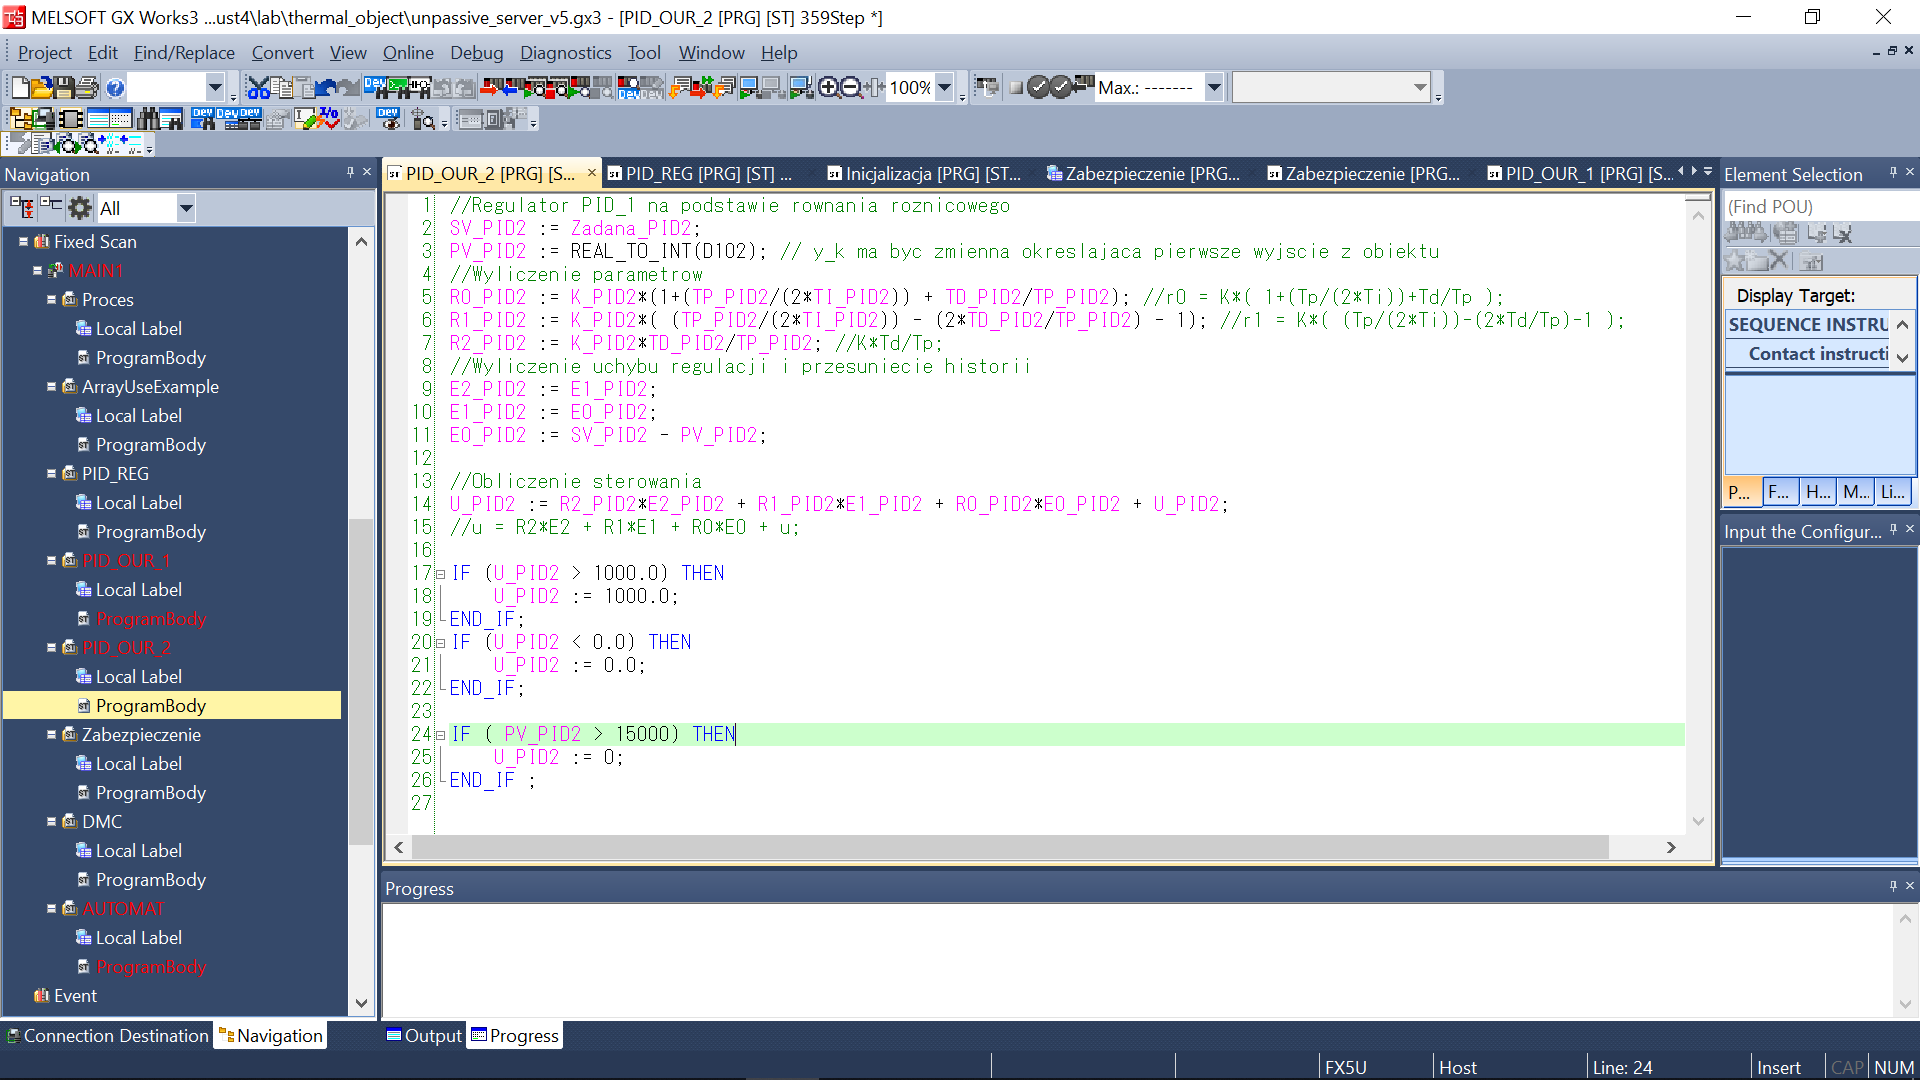
\includegraphics[scale=0.45]{sections/thermal/DrzewkoZFolderami.png}
\caption{Zrzut ekranu pokazujący strukturę elementu Fixed Scan}
\end{figure}


\section{Wyniki działania algorytmu regulacji}
\label{thermal_pid_wyniki}

\subsection{Pierwsza próba}
\label{thermal_pid_proba_1}
Podczas pierwszego eksperymentu skupiliśmy się mocniej na sprawdzeniu działania komunikacji z stanowiskiem, pracy obiektu oraz funkcjonowaniu zaimplementowanego algorytmu regulacji (np. czy sterowania nie przekraczają ograniczeń) niż na dobieraniu wartości nastawów. Z tego powodu zastosowaliśmy regulator P z wzmocnieniem równym 1 dla obu regulatorów jednowymiarowych. Jak możemy zobaczyć na wykresach \ref{lab_pid_1_out} wyjścia procesu wielowymiarowego charakteryzują się bardzo dużym uchybem ustalonym. Przebiegi sygnałów sterujących możemy zaobserwować na rysunkach \ref{lab_pid_1_in} charakteryzują się one oscylacjami. Otrzymane rezultaty oczywiście nas nie satysfakcjonowały, jednak ta próba miała służyć czemuś zupełnie innemu. Chcieliśmy głównie sprawdzić w jaki sposób prawidłowo dokonywać eksperymentów i pomiarów z użyciem sterownika PLC, ponieważ jego zastosowanie było dla nas nowością. W następnych eksperymentach skupiliśmy się już w pełni na dobieraniu nastawów regulatorów. 

%% wyjscia 

\begin{figure}
    \centering
    \begin{subfigure}[b]{\textwidth}
        \centering
        \resizebox{\linewidth}{!}{
            \begin{tikzpicture}
                \begin{axis}[
                    width=0.98\textwidth,
                    height=7cm,
                    xmin=0.0,xmax=500,ymin=25,ymax=41,
                    xlabel={$k$},
                    ylabel={$y_{\mathrm{1}}[k]$},
                    legend pos=south east,
                    y tick label style={/pgf/number format/1000 sep=},
                    ] 
                    \addlegendentry{$y_{\mathrm{1}}[k]$},
                    \addlegendentry{$y_{\mathrm{1}}^{\mathrm{zad}}[k]$},
                
                    \addlegendimage{no markers,red}
                    \addlegendimage{no markers,blue}
                
                    \addplot[red, semithick] file{../lab/thermal_object/PID/PROBA1output_1.csv};  
                    \addplot[blue, semithick] file{../lab/thermal_object/PID/PROBA1stpt_1.csv};
                    
                    \end{axis}
            \end{tikzpicture}
        }
        \end{subfigure}

        \begin{subfigure}[b]{\textwidth}
            \centering
            \resizebox{\linewidth}{!}{
                \begin{tikzpicture}
                    \begin{axis}[
                        width=0.98\textwidth,
                        height=7cm,
                        xmin=0.0,xmax=500,ymin=25,ymax=41,
                        xlabel={$k$},
                        ylabel={$y_{\mathrm{2}}[k]$},
                        legend pos=south east,
                        y tick label style={/pgf/number format/1000 sep=},
                        ] 
                        \addlegendentry{$y_{\mathrm{2}}[k]$},
                        \addlegendentry{$y_{\mathrm{2}}^{\mathrm{zad}}[k]$},
                    
                        \addlegendimage{no markers,red}
                        \addlegendimage{no markers,blue}
                    
                        \addplot[red, semithick] file{../lab/thermal_object/PID/PROBA1output_2.csv};  
                        \addplot[blue, semithick] file{../lab/thermal_object/PID/PROBA1stpt_2.csv};
                        
                        \end{axis}
                \end{tikzpicture}
            }
        \end{subfigure}
        \caption{Wyjścia procesu wielowymiarowego}
        \label{lab_pid_1_out}

\end{figure}

%% wejscia 

\begin{figure}
    \centering
    \begin{subfigure}[b]{\textwidth}
        \centering
        \resizebox{\linewidth}{!}{
            \begin{tikzpicture}
                \begin{axis}[
                    width=0.98\textwidth,
                    height=6cm,
                    xmin=0.0,xmax=500,%ymin=-3,ymax=3,
                    xlabel={$k$},
                    ylabel={$u_{\mathrm{1}}[k]$},
                    legend pos=south east,
                    y tick label style={/pgf/number format/1000 sep=},
                    ] 
                    \addlegendentry{$u_{\mathrm{1}}[k]$},
                    \addlegendimage{no markers,blue}
                    \addplot[const plot, blue, semithick] file{../lab/thermal_object/PID/PROBA1input_1.csv};  
                \end{axis}
            \end{tikzpicture}
        }
    \end{subfigure}

    \begin{subfigure}[b]{\textwidth}
        \centering
        \resizebox{\linewidth}{!}{
            \begin{tikzpicture}
                \begin{axis}[
                    width=0.98\textwidth,
                    height=6cm,
                    xmin=0.0,xmax=500,%ymin=-3,ymax=3,
                    xlabel={$k$},
                    ylabel={$u_{\mathrm{2}}[k]$},
                    legend pos=south east,
                    y tick label style={/pgf/number format/1000 sep=},
                    ] 
                    \addlegendentry{$u_{\mathrm{2}}[k]$},
                    \addlegendimage{no markers,blue}
                    \addplot[const plot, blue, semithick] file{../lab/thermal_object/PID/PROBA1input_2.csv};  
                \end{axis}
            \end{tikzpicture}
        }
    \end{subfigure}

    
    \caption{Wejścia procesu wielowymiarowego}
    \label{lab_pid_1_in}
\end{figure}
\FloatBarrier

\subsection{Druga próba}
\label{thermal_pid_proba_2}
W tej próbie do regulacji obiektu użyliśmy dwupętlowego regulatora PID, którego nastawy regulatorów jednowymiarowych były równe $K_{\mathrm{r}} = 40$, $T_{\mathrm{i}} = 200$, $ T_{\mathrm{d}} = 10$. Przebiegi wyjścia procesu możemy zobaczyć na rysunkach \ref{lab_pid_2_out}. Po ich przeanalizowaniu widzimy, że wartość $40$ została osiągnięta dla obu wyjść w okolicach próbki $k=500$. W tym miejscu również wyraźnie wygasły oscylacje, które na początku regulacji były spore. Po $500$ próbce dokonaliśmy zmiany wartości zadanej dla pierwszego wyjścia. Wielkość ta została osiągnięta całkiem szybko i sygnał z wyjścia procesu zaczął się stabilizować wokół nowej wartości zadanej. Zmiana ta nie miała dużego wpływu na regulację wyjścia drugiego. Wejścia procesu wielowymiarowego w niektórych momentach osiągają ograniczenia i przez pewien czas regulacji charakteryzują się łagodnymi oscylacjami, które z czasem się stabilizują. Wartości nastawów są wielkościami uzyskanymi po dostrojeniu regulatora PID w czasie pierwszych laboratoriów. Wartości te sprawdziły się również procesu wielowymiarowego. Przy ocenie działania regulatora wzięliśmy również pod uwagę fakt, że obiektem regulacji jest rzeczywiste stanowisko, które zawsze wprowadza pewne zakłócenia i jest trudniejsze w dobraniu nastawów dla regulatorów. 

%% wyjscia 

\begin{figure}
    \centering
    \begin{subfigure}[b]{\textwidth}
        \centering
        \resizebox{\linewidth}{!}{
            \begin{tikzpicture}
                \begin{axis}[
                    width=0.98\textwidth,
                    height=7cm,
                    xmin=0.0,xmax=1000,ymin=31,ymax=48,
                    xlabel={$k$},
                    ylabel={$y_{\mathrm{1}}[k]$},
                    legend pos=south east,
                    y tick label style={/pgf/number format/1000 sep=},
                    ] 
                    \addlegendentry{$y_{\mathrm{1}}[k]$},
                    \addlegendentry{$y_{\mathrm{1}}^{\mathrm{zad}}[k]$},
                
                    \addlegendimage{no markers,red}
                    \addlegendimage{no markers,blue}
                
                    \addplot[red, semithick] file{../lab/thermal_object/PID/PROBA2output_1.csv};  
                    \addplot[blue, semithick] file{../lab/thermal_object/PID/PROBA2stpt_1.csv};
                    
                    \end{axis}
            \end{tikzpicture}
        }
        \end{subfigure}

        \begin{subfigure}[b]{\textwidth}
            \centering
            \resizebox{\linewidth}{!}{
                \begin{tikzpicture}
                    \begin{axis}[
                        width=0.98\textwidth,
                        height=7cm,
                        xmin=0.0,xmax=1000,ymin=31,ymax=46,
                        xlabel={$k$},
                        ylabel={$y_{\mathrm{2}}[k]$},
                        legend pos=south east,
                        y tick label style={/pgf/number format/1000 sep=},
                        ] 
                        \addlegendentry{$y_{\mathrm{2}}[k]$},
                        \addlegendentry{$y_{\mathrm{2}}^{\mathrm{zad}}[k]$},
                    
                        \addlegendimage{no markers,red}
                        \addlegendimage{no markers,blue}
                    
                        \addplot[red, semithick] file{../lab/thermal_object/PID/PROBA2output_2.csv};  
                        \addplot[blue, semithick] file{../lab/thermal_object/PID/PROBA2stpt_2.csv};
                        
                        \end{axis}
                \end{tikzpicture}
            }
        \end{subfigure}
        \caption{Wyjścia procesu wielowymiarowego}
        \label{lab_pid_2_out}

\end{figure}

%% wejscia 

\begin{figure}
    \centering
    \begin{subfigure}[b]{\textwidth}
        \centering
        \resizebox{\linewidth}{!}{
            \begin{tikzpicture}
                \begin{axis}[
                    width=0.98\textwidth,
                    height=6cm,
                    xmin=0.0,xmax=1000,%ymin=-3,ymax=3,
                    xlabel={$k$},
                    ylabel={$u_{\mathrm{1}}[k]$},
                    legend pos=south east,
                    y tick label style={/pgf/number format/1000 sep=},
                    ] 
                    \addlegendentry{$u_{\mathrm{1}}[k]$},
                    \addlegendimage{no markers,blue}
                    \addplot[const plot, blue, semithick] file{../lab/thermal_object/PID/PROBA2input_1.csv};  
                \end{axis}
            \end{tikzpicture}
        }
    \end{subfigure}

    \begin{subfigure}[b]{\textwidth}
        \centering
        \resizebox{\linewidth}{!}{
            \begin{tikzpicture}
                \begin{axis}[
                    width=0.98\textwidth,
                    height=6cm,
                    xmin=0.0,xmax=1000,%ymin=-3,ymax=3,
                    xlabel={$k$},
                    ylabel={$u_{\mathrm{2}}[k]$},
                    legend pos=south east,
                    y tick label style={/pgf/number format/1000 sep=},
                    ] 
                    \addlegendentry{$u_{\mathrm{2}}[k]$},
                    \addlegendimage{no markers,blue}
                    \addplot[const plot, blue, semithick] file{../lab/thermal_object/PID/PROBA2input_2.csv};  
                \end{axis}
            \end{tikzpicture}
        }
    \end{subfigure}

    
    \caption{Wejścia procesu wielowymiarowego}
    \label{lab_pid_2_in}
\end{figure}
\FloatBarrier

\subsection{Trzecia próba}
\label{thermal_pid_proba_3}
Widząc z jaką łatwością nasze poprzednie regulatory wpadały w oscylację postanowiliśmy zmniejszyć wielkość wzmocnienie regulatorów. Nastawy dla tej próby prezentują się następująco $K_{\mathrm{r}} = 20$, $T_{\mathrm{i}} = 200$, $ T_{\mathrm{d}} = 10$. 
\\ \indent  Tym razem dokonaliśmy następujących zmian wielkości zadanej, wartości przed rozpoczęciem pomiaru: $y_{\mathrm{1}}^{\mathrm{zad}}[k] = 43^{\circ} C$ i $y_{\mathrm{2}}^{\mathrm{zad}}[k] = 37^{\circ} C$, wartości które chcieliśmy osiągnąć:  $y_{\mathrm{1}}^{\mathrm{zad}}[k] = \num{35.3}^{\circ} C$ i $y_{\mathrm{2}}^{\mathrm{zad}}[k] = 45^{\circ} C$. Chcieliśmy zobaczyć czy przy osiąganiu mniejszych wartości zadanych regulator również zachowa się poprawnie. Na rysunkach \ref{lab_pid_3_out} możemy zauważyć jak szybko jest osiągana wartość zadana. Jej zmiana nastąpiła na chwilę przed próbką $0$. Otrzymane rezultaty są nawet lepsze niż te osiągane podczas drugiej próby. Wyjścia procesu bardzo szybko stabilizują się wokół wartości zadanej. Przebiegi sygnałów wejścia procesu również są bardzo stabilne, dzięki czemu elementy wykonawcze urządzeń bezpośrednio oddziałujących na obiekt nie są narażone na wysokie skoki sterowań. Uznaliśmy, że nastawy te z powodzeniem mogą regulować stanowiskiem chłodząco-grzejącym i przeszliśmy do implementacji regulatora DMC.

%% wyjscia 

\begin{figure}
    \centering
    \begin{subfigure}[b]{\textwidth}
        \centering
        \resizebox{\linewidth}{!}{
            \begin{tikzpicture}
                \begin{axis}[
                    width=0.98\textwidth,
                    height=7cm,
                    xmin=0.0,xmax=1000,%ymin=25,ymax=41,
                    xlabel={$k$},
                    ylabel={$y_{\mathrm{1}}[k]$},
                    legend pos=north east,
                    y tick label style={/pgf/number format/1000 sep=},
                    ] 
                    \addlegendentry{$y_{\mathrm{1}}[k]$},
                    \addlegendentry{$y_{\mathrm{1}}^{\mathrm{zad}}[k]$},
                
                    \addlegendimage{no markers,red}
                    \addlegendimage{no markers,blue}
                
                    \addplot[red, semithick] file{../lab/thermal_object/PID/PROBA3output_1.csv};  
                    \addplot[blue, semithick] file{../lab/thermal_object/PID/PROBA3stpt_1.csv};
                    
                    \end{axis}
            \end{tikzpicture}
        }
        \end{subfigure}

        \begin{subfigure}[b]{\textwidth}
            \centering
            \resizebox{\linewidth}{!}{
                \begin{tikzpicture}
                    \begin{axis}[
                        width=0.98\textwidth,
                        height=7cm,
                        xmin=0.0,xmax=1000,%ymin=25,ymax=41,
                        xlabel={$k$},
                        ylabel={$y_{\mathrm{2}}[k]$},
                        legend pos=south east,
                        y tick label style={/pgf/number format/1000 sep=},
                        ] 
                        \addlegendentry{$y_{\mathrm{2}}[k]$},
                        \addlegendentry{$y_{\mathrm{2}}^{\mathrm{zad}}[k]$},
                    
                        \addlegendimage{no markers,red}
                        \addlegendimage{no markers,blue}
                    
                        \addplot[red, semithick] file{../lab/thermal_object/PID/PROBA3output_2.csv};  
                        \addplot[blue, semithick] file{../lab/thermal_object/PID/PROBA3stpt_2.csv};
                        
                        \end{axis}
                \end{tikzpicture}
            }
        \end{subfigure}
        \caption{Wyjścia procesu wielowymiarowego}
        \label{lab_pid_3_out}

\end{figure}

%% wejscia 

\begin{figure}
    \centering
    \begin{subfigure}[b]{\textwidth}
        \centering
        \resizebox{\linewidth}{!}{
            \begin{tikzpicture}
                \begin{axis}[
                    width=0.98\textwidth,
                    height=6cm,
                    xmin=0.0,xmax=1000,%ymin=-3,ymax=3,
                    xlabel={$k$},
                    ylabel={$u_{\mathrm{1}}[k]$},
                    legend pos=north east,
                    y tick label style={/pgf/number format/1000 sep=},
                    ] 
                    \addlegendentry{$u_{\mathrm{1}}[k]$},
                    \addlegendimage{no markers,blue}
                    \addplot[const plot, blue, semithick] file{../lab/thermal_object/PID/PROBA3input_1.csv};  
                \end{axis}
            \end{tikzpicture}
        }
    \end{subfigure}

    \begin{subfigure}[b]{\textwidth}
        \centering
        \resizebox{\linewidth}{!}{
            \begin{tikzpicture}
                \begin{axis}[
                    width=0.98\textwidth,
                    height=6cm,
                    xmin=0.0,xmax=1000,%ymin=-3,ymax=3,
                    xlabel={$k$},
                    ylabel={$u_{\mathrm{2}}[k]$},
                    legend pos=south east,
                    y tick label style={/pgf/number format/1000 sep=},
                    ] 
                    \addlegendentry{$u_{\mathrm{2}}[k]$},
                    \addlegendimage{no markers,blue}
                    \addplot[const plot, blue, semithick] file{../lab/thermal_object/PID/PROBA3input_2.csv};  
                \end{axis}
            \end{tikzpicture}
        }
    \end{subfigure}

    
    \caption{Wejścia procesu wielowymiarowego}
    \label{lab_pid_3_in}
\end{figure}
\FloatBarrier